\documentclass[12pt]{article}
\usepackage{mandi}
\usepackage{braket}
\usepackage{graphicsx}
\usepackage{amsmath}
\usepackage{amsthm,amssymb, mathtools}
\usepackage{amsfonts}
\usepackage{tikz}
\usepackage{epstopdf}
\tolerance=1
\emergencystretch=\maxdimen
\hyphenpenalty=10000
\hbadness=10000
% Palatino font (ppl must be installed).
\renewcommand*\rmdefault{ppl}
% Iwona font (iwona must be installed).
%\renewcommand*\rmdefault{iwona}
\newtheorem{theorem}{Theorem}
\DeclarePairedDelimiter\norm\lVert\rVert
\begin{document}
\title{Implementation of Quantum Computing Techniques on NMR systems}
\author{Anurag Pallaprolu \\ 2012B5A3405P \\ BITS Pilani }
\maketitle
\begin{abstract}
This document is submitted as a partial requirement for the course Quantum Information and Computing, BITS Pilani. The phenomenon of NMR can be used to generate spin states of nuclei and these can be used as qubits for computational purposes, the speciality being, an ensemble of molecules must be utilized. According to ~\cite{JAJ}, it is both the best, and the worst technologies in quantum computing, reasons being the ease at which unitary quantum gates can be implemented and the difficulty in exact measurements without disturbing the ensemble respectively. 
\end{abstract}
\clearpage
\tableofcontents
\setcounter{tocdepth}{3}
\clearpage
\section{Introduction}
\textbf{Nuclear Magnetic Resonance} is an important phenomenon in Physics, Chemistry and Medicine, was first discovered by \textbf{Isaac Isidor Rabi} in 1938, for which he won the Nobel Prize in 1944. Later, \textbf{Edward Mills Purcell} and \textbf{Felix Bloch} won the 1952 Nobel Prize \textit{for their developments of new methods for nuclear magnetic precision measurements and discoveries in connection therewith}.~\cite{npb}. The phenomenon occurs to certain nuclei, when placed in a strong static magnetic field, and are exposed to an oscillating magnetic field, depending on whether the nuclei possess intrinsic nucleonic spin or not. The concept of spin is quite simple as explained in the accompanying document ~\cite{me} and a fact that must be kept in mind is that we are talking about quantum mechanical version of spin and hence, we would be looking at things like Zeeman Effect etc,. When placed in a magnetic field of frequency $\mathbb{B}$, a particle with some net non-zero spin can absorb a photon of frequency $\nu$. The relationship being $$\nu = \gamma\mathbb{B}$$ The number $\gamma$ is called as the \textbf{gyromagnetic ratio} and depends on the particle at hand ~\cite{jph}. Simply seen, when any particle with a non zero spin is placed in a static magnetic field, it can stay in two energy levels, the lower energy level due to the straight pairing of N-S poles of the field to that of the particle, and the higher \textit{unstable} energy state of the anti-pairing of the N-S poles of the field with the particle.
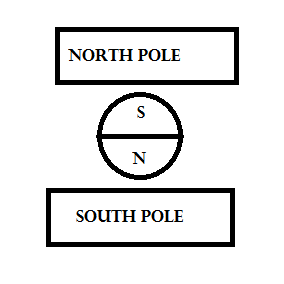
\includegraphics[scale=0.9]{nsns.png}
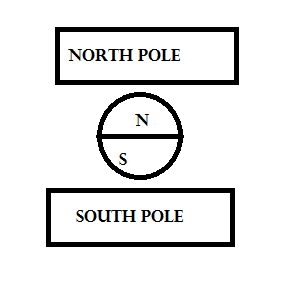
\includegraphics[scale=0.9]{nnss.png}

As we have seen, any transition from these two energy levels must be facilitated by quanta, according to Planck's hypothesis. Hence, we get the relation
$$E = h\gamma\mathbb{B}$$
When there is a lower level transition, or a photon arrives with the frequency equal to the \textbf{Larmor Frequency} given before, then a shift in the energy level happens~\cite{acadml}. In the case of \textbf{nuclear} magnetic resonance, the emission of photons or the absorbed photon usually lie in the radio frequency ranges of the electromagnetic spectrum. In NMR spectroscopy, $\nu$ is between 60 and 800 MHz for hydrogen nuclei. In clinical MRI, $\nu$ is typically between 15 and 80 MHz for hydrogen imaging ~\cite{jph}. The simplest possible implementation of NMR in actual atoms is the \textbf{Continuous Wave} NMR experiment. In this, you can either hold the magnetic field constant and supply RF pulses with varying frequency to note the absorbed energy, or, you can hold the pulsing frequency constant and vary the magnetic field to look for some resonance. The diagrams below should be helpful in making this point clear.

\begin{figure}
\begin{tikzpicture}[overlay]
\draw [<->,thick] (0,5) node (yaxis) [below] {Absorbed Energy}
        |- (5,0) node (xaxis) [right] {Frequency};
\draw [ultra thick, red] (0,0) -- (3,0)--(4,3)--(5,0)--(6,0);        
\end{tikzpicture}
\caption{The Energy-Frequency Diagram}
\end{figure}
\begin{figure}
\begin{tikzpicture}
\draw [<->,thick] (0,5) node (yaxis) [above] {Energy}
        |- (5,0) node (xaxis) [right] {Magnetic Field};

\draw (0,2.5) -- (4,4) --(6,4);
\draw (0,2.5) -- (4,1.5) --(6,1.5);
\draw [ultra thick, red] (3,1) -- (3,4);
\node [above] at (6,4) {Unpaired High Energy};
\node [above] at (6,1.5) {Paired High Energy};
\end{tikzpicture}
\caption{CWNMR Frequency Variation}
\end{figure}
\clearpage
\subsection{Ensemble}
Now, we shall move on to statistics of the spin particle ensembles. The problem with NMR spectroscopy is that the radio frequency photons are hard to detect, identify and measure as each one of them carries an energy of around $1\mu eV$. This leads to the following idea that, inorder to measure significant readings, an \textbf{ensemble} is required to be used experimentally. The number of molecules is approximated to be of the order of $10^{19}$ according to ~\cite{JAJ}. To analyze such large systems, we must comply to look at the \textit{macroscopic} point of view rather than the \textit{microscopic} one, and hence, we shall look at a bit of \textbf{Boltzmann statistics}. It is based on the probabilistic law that \textbf{Ludwig Boltzmann} proposed, and is very well explained in the standard ~\cite{Feyn}. We define $$\beta = \frac{1}{kT}$$ and then we can state from Boltzmann's law, that, 
$$\frac{N^{+}}{N^{-}} = e^{-\beta E}$$ where $N^+$ and $N^-$ are the number of particles in spin up and down states respectively and E is the energy difference between the two states. 
\begin{figure}
\begin{center}
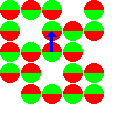
\includegraphics[scale=1]{ens1.png}
\end{center}
\caption{The Spin Packet of an Ensemble and the net $\mathbb{M}$ vector}
\end{figure}
Then, we take an ensemble and compartmentalize it into smaller boxes and call these \textbf{spin packets}. This then leads to the formulation of a magnetization vector $\mathbb{M}$ for each of these packets and it is obvious that $$\mathbb{M} =  \lambda (N^+ - N^-)$$ A system of axes can be set up here, with the z axis in the direction of $\mathbb{M}$. Let us take a deviation here, and look at the contributing Hamiltonian to NMR processes. According to the excellent paper ~\cite{ohio}, any atomic hamiltonian contains \textbf{nine important} terms that relate to any type of a quantum process. Let us look at them one by one. 
\clearpage
\subsection{The Atomic Hamiltonian}
The first one is called the \textbf{electronic Hamiltonian}, which is essentially a combination of all Coulombic potentials and kinetic energies
$$\mathcal{H}_{elec} = \sum_i \frac{{p_i}^{2}}{2m} - \sum_{i,j} \frac{z_je^2}{r_{ij}} + \sum_{i,j} \frac{e^2}{r_{ij}}$$
The next term is the \textbf{crystal field hamiltonian}, which deals with the interaction of electrons with the ions trapped in a crystal lattice. It also has a Coulombic form 
$$\mathcal{H}_{CF} = -\sum_{i,j} \frac{Q_je}{r_{ij}}$$
The third term is of great importance in particle physics, it is the \textbf{spin-orbit coupling hamiltonian}, which is of the form of 
$$\mathcal{H}_{SO} = \mu \mathbb{L}\mathbb{S}$$
where $\mathbb{L}$ and $\mathbb{S}$ are the orbital and spin angular momentum terms, respectively and $\mu$ is the \textbf{coupling constant} of the interaction, a term more commonly used in determining the extent of a force field in any quantum field theory. We shall not go deeper here. The next term, please. They are the \textbf{Zeeman Terms} which play an important role in describing, not only NMR but also another similar phenomenon by the name of \textbf{Electron Spin Resonance} or simply \textbf{ESR}.
$$H_{ESR} = \beta\vectdotvect{\mathbb{B}}{(\textbf{L}+\textbf{S})}$$
$$H_{NMR} = \mathcal{G}_{i}^n\beta^nB_{k}{\mathcal{N}^{ik}}$$
Here and henceforth, we will be using the Einstein summation convention of summing over repeated indices wherever found(the \textit{upstairs sums downstairs rule}). In the above equation $\mathcal{N}^{ik}$ is the $k$th component of the $i$th nucleus' magnetic moment. Indices which are not stairwise complementary are just for representation and are \textbf{not} summed over(like $n$ int the above equation).
The next hamiltonian is one that is important to NMR Computing, it is the \textbf{nuclear interaction hamiltonian}.
$$H_{NN} = \frac{1}{2}\mathcal{N}^\mu \mathcal{J}_{\mu \nu} \mathcal{N}^\nu $$
Here, the term $\mathcal{J}$ is a \textbf{tensorial} term representing the coupling coefficient between the two nuclei. More on this will be explained when we are looking at \textbf{qubit tensor product implementations} in NMR computers. The other three hamiltonians \textbf{the hyperfine splitting hamiltonian, spin-spin interaction hamiltonian, and the quadrupolar energy} are not exactly important here, and hence, I shall give references where it is explained much better.
Summarizing, any atomic hamiltonian will be of the form:
$$\mathcal{H}_{atom} = \sum_i \frac{{p_i}^{2}}{2m} - \sum_{i,j} \frac{z_je^2}{r_{ij}} + \sum_{i,j} \frac{e^2}{r_{ij}} -\sum_{i,j} \frac{Q_je}{r_{ij}} +\mu \mathbb{L}\mathbb{S} +  \beta\vectdotvect{\mathbb{B}}{(\textbf{L}+\textbf{S})} + \mathcal{G}_{i}^n\beta^nB_{k}{\mathcal{N}^{ik}} + \frac{1}{2}\mathcal{N}^\mu \mathcal{J}_{\mu \nu} \mathcal{N}^\nu $$
This equation is something big, and a few definitive \textit{relativistic} corrections~\cite{dirac} will make this theory complete.
\clearpage
\section{A Quick and Dirty Introduction to Quantum Computing Terminologies}
\subsection{Qubit}
I shall start out by explaining what a quantum bit or a \textbf{qubit} is. The name is self explanatory. Let me just point out the crucial difference, a classical bit can, at any point of time, take only one of the two quantized boolean states. Quantum bits on the other hand can be in a simultaneous superposition state of the individual quantized values. To put it symbolically,
\begin{center}
IN CLASSICAL COMPUTATION
\end{center}
$$\Ket{0}, \Ket{1}$$
\begin{center}
IN QUANTUM COMPUTATION
\end{center}
$$\frac{\Ket{0}+\Ket{1}}{\sqrt{2}}$$
 The $\sqrt{2}$ factor is completely arbitrary. In general, the two ket states might have any arbitrary (normalized) amplitudes. The behavior of these states is governed by the laws of quantum mechanics. That's all there is for a qubit. Now let us look at a few operations on qubits. They exist in vector spaces(more on this later) and can be operated on any two vectors. They could also be operated on each other using any standard vector arithmetic. An inner product can be established on the vector space in which the kets exist(more on this later).  The first question that might occur to any opportunistic person would be to expand this amalgamated state to more than one bit. This can be done due to the wonderful mathematical process of taking the \textbf{tensor product} or the \textbf{Kronecker product} of two or more qubits. The idea is quite simple and is exactly like the \textbf{direct product of two sets}. 
$$\frac{\Ket{0}+\Ket{1}}{\sqrt{2}}\otimes\frac{\Ket{0}-\Ket{1}}{\sqrt{2}} = \frac{1}{\sqrt{2}}(\Ket{00}-\Ket{01}+\Ket{10}-\Ket{11})$$
Your first thought might be, what in the world is $$\Ket{00}$$Well, don't get bewildered. Just think of it as a larger ket vector tracing two smaller qubit ket components. Let us talk about quantum gates to make this concept clear. 
\subsection{Quantum Gate}
A \textbf{gate} in any device is in general a logical unit which operates on Boolean variables. A \textbf{quantum gate} is a device which operates on \textit{quantum} boolean variables. I have to state a few facts before going into the explanation of the workings of a quantum gate. Every quantum mechanical operation takes one ket from the \textbf{Hilbert Space} in which it exists to another one with the help of a (matrix) transformation called as a \textbf{unitary transformation}. You might have heard of unitary matrices. Well, according to linear algebra, any linear transformation on a vector can be represented by a \textbf{matrix of transformation}. If this matrix turns out to be unitary, a situation which is most favorable for representing changes in quantum ket states, then it is a unitary transformation. This is a very bare bones version of one of the postulates of quantum mechanics. For a fuller explanation, refer to any standard quantum text like \textit{Griffiths}, \textit{Sakurai} or \textit{Shankar}. Anyway, any operation on a ket can be seen as a unitary matrix operating on its vector representation. Now, gates also operate on kets/qubits. Hence, the moral of the above story is that \textbf{every quantum gate can be represented in its unitary matrix representation}. For example, look at the simple circuit below,\\
\begin{center}
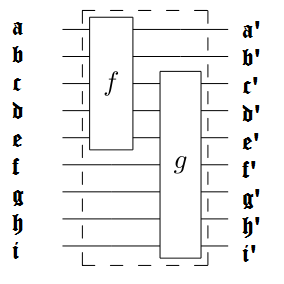
\includegraphics[scale=0.8]{qgate1.png}
\end{center}
The input lines all carry one qubit each. The gate $f$ operates on the first five lines and then the $g$ gate operates on the last seven lines. The input can be seen as a tensor product multi-qubit of 9 single qubits represented compactly as
$$\Ket{\Psi} = \bigotimes_{x=a}^{x=i}\Ket{x}$$ For instance, if each of the inputs was $\Ket{0}$, then $\Ket{\Psi} = \bigotimes_{x=a=0}^{x=i=0}\Ket{0}=\Ket{000000000}$. As discussed before, \textit{the operation of the $f$ gate can be represented by a unitary transformation on the initial (multi)ket}. Let us call this matrix as $\mathcal{F}$. Then the next state of the combined qubit after the $\mathcal{F}$  would then be $$\mathcal{F}\bigotimes_{x=f,x'=a}^{x=i,x'=e}\Ket{x'}\Ket{x} = \bigotimes_{x=f,x'=a}^{x=i,x'=e}\mathcal{F}\Ket{x'}\Ket{x}$$ Note the change in the indices of summation as not all individual qubits are going through $\mathcal{F}$. Let's call the multiqubit at this step as $\Ket{\Psi_{1}}$.The next step would be to operate $g$ onto the qubits $c$ through $i$. Let's call its matrix as $\mathcal{G}$. The qubit at this stage would be $$\mathcal{G}\Ket{\Psi_{1}} =  \bigotimes_{x=f,x'=a}^{x=i,x'=e}\mathcal{F}\Ket{x'}\mathcal{G}\Ket{x}$$
$$\bigotimes_{x=f,x'=a}^{x=i,x'=e}\mathcal{F}\Ket{x'}\mathcal{G}\Ket{x} = \bigotimes_{x=a'}^{x=i'}\Ket{x}$$
The concept of parallelism should get a bit clear now as you can clearly see the individual operation of gates on qubit, but the final (unnormalized) state is correlated. This should also point out one of the major issues with parallelism theory, \textit{we can compute a state in \textbf{one} step which contains, say, the values of the function $f(x)$ for many values of $x$(whereas a classical computer would take $n$ steps where $n$ is the number of values of $x$). But to access the values, we have to perform a measurement, and a measurement performed on a particular $\Ket{x}$ would lead to the \textbf{collapse of the ket at the value}}. The last line quantum mechanically tells us that we would lose information about all other values of $x$  but retain the value of $f(x_{measured})$. This might sound like quantum computing just lost a point against its classical opponent, but where it wins is (for example, it is apparent in \textbf{Deutsch's Algorithm}) the final state can be a combination of operated individual values, like $f(x_1)+f(x_2)$ etc., which the classical computer \textbf{would still take $n$ steps to do(in the present case 2)}. You can read up more on standard quantum gates from ~\cite{mni} but I think this discussion shall suffice for the documentation.
\subsection{Walsh-Hadamard Transform}
However, I shall describe one specific type of gate, called the \textbf{Hadamard Gate} named after Jacques Hadamard. It is represented by the symbol 
\begin{center}
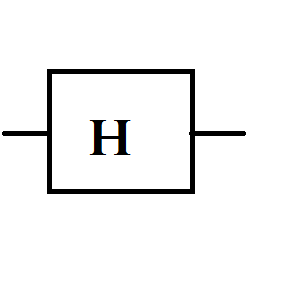
\includegraphics[scale=0.5]{qhad.png}
\end{center}
Simply put, let us take any qubit in the standard basis of $\mathbb{H}$ say $\Ket{\psi} = \alpha\Ket{0} + \beta\Ket{1}$. The operation of $\mathcal{H}$ on standard basis qubits is known $$\mathcal{H}\Ket{0} = \frac{\Ket{0}+\Ket{1}}{\sqrt{2}}$$
$$\mathcal{H}\Ket{1} = \frac{\Ket{0}-\Ket{1}}{\sqrt{2}}$$
With this, now we can see
$$\mathcal{H}\Ket{\psi} = \alpha\frac{\Ket{0}+\Ket{1}}{\sqrt{2}} + \beta\frac{\Ket{0}-\Ket{1}}{\sqrt{2}} = \frac{\alpha + \beta}{\sqrt{2}}\Ket{0} + \frac{\alpha - \beta}{\sqrt{2}}\Ket{1}$$
Hence, as you can see, the operation is quite simple, and one can easily derive the transformation matrix of $\mathcal{H}$. Now, let us take two qubits, for simplicity, let both of them be $\Ket{0}$. Now, let us apply the \textbf{Hadamard Gate on 2 Qubits or the Nth order Hadamard Gate} represented by $\mathcal{H}^{\bigotimes 2}$. This is nothing but the operator $\mathcal{H}\bigotimes\mathcal{H}$. Thus, two Hadamard gates operate on individual qubits and are again \textit{tensorially} combined into one qubit. Note the pattern of $\mathcal{H}^{\bigotimes n}$ as $n$ increases, as given below.
$$\mathcal{H}^{\bigotimes 2}\Ket{00} = \mathcal{H}\Ket{0}\mathcal{H}\Ket{0} = \frac{\Ket{00}+\Ket{01}+\Ket{10}+\Ket{11}}{2}$$
$$\mathcal{H}^{\bigotimes 3}\Ket{000} = \frac{\Ket{000}+\Ket{001}+....+\Ket{101}+\Ket{111}}{2^{3/2}}$$ Notice how all the binary numbers upto $2^n$ are being listed in the combined multikets. This general Hadamard Transform of $n$ qubits can be combined mathematically as
$$\mathcal{H}^{\bigotimes n}\Ket{0^n} = \sum_{x=0}^{x=2^n-1}\frac{\Ket{x}}{\sqrt{2^n}}$$ This operation is much more generally known as the \textbf{Walsh-Hadamard Transform} and comes under a general class of such summable or integrable transforms known as \textit{Fourier Transforms}, which can be proven to be convergent and are applicable for discontinuous functions as well(\textit{Dirichlet's Theorem}), but we shall not go into this much deep. The development of the neccesary tools is complete, we shall start our progress in the implementation of quantum computing systems in NMR experiments.
\clearpage
\section{Implementation}
\subsection{The Bloch Vectors, The Ket and The $\mathbb{SU}(2)\cong\mathbb{SO}(3)$ theorem}
To look at the implementation schema, we must first look at a bit of \textbf{representation} theory first. The aim of this section is to explain the proof given in the appendix of ~\cite{ohio}. In quantum mechanics, we work with \textbf{kets} present in a Hilbert space $\mathbb{H}$. Any picture used, either the wave mechanical perspective or the matrix mechanical perspective, has the concept of state vectors. The entire idea of a representation is to simplify the way we look at terms and symmetries. It is easy to establish a \textbf{homomorphism} between the state vector concept and the \textbf{density matrix formulation} and this shall not be proven in the document. However, we can also prove another mapping. The homomorphism between the standard \textbf{Lie Groups} $\mathbb{SO}(3)$ and $\mathbb{SU}(2)$. In quantum computing, a qubit state can be represented always in the following form $$\ket{\psi} = \cos\frac{\theta}{2}\ket{0}+e^{i\phi}\sin\frac{\theta}{2}\ket{1}$$ This is called the \textbf{Bloch Vector representation}. Given the values of $\theta, \phi$ we can always represent the qubit on a unit sphere called the \textbf{Bloch-Poincare sphere}. The homomorphism that we are going to prove will ensure that operating on Bloch vectors using \textbf{rotation matrices} is the same as operating on ket state vectors using \textbf{unitary hermitian matrices}. That is, 
$$\hat{U}\ket{\psi} = \cos\frac{\theta}{2}\hat{U}\ket{0} + e^{i\phi}\sin\frac{\theta}{2}\hat{U}\ket{1}$$
$$\vec{v'_B}(\theta,\phi) = \mathbb{R}\vec{v_B}(\theta, \phi)$$
Clearly, both $\hat{U}$ and $\mathbb{R}$ are members of the Lie groups $\mathbb{SU}(2)$ and $\mathbb{SO}(3)$(Special Unitary group of unitary matrices of order 2 and Special Orthogonal group of orthogonal matrices of order 3 respectively). We need to find $\mathbb{R}(\hat{U})$. If we can choose $$\mathbb{R}(\hat{U})_{ij} = \frac{1}{2}\mathrm{Tr}(\sigma_i\hat{U}\sigma_j\hat{U^-1})$$ then, by simple verification, our problem is solved. The intuition behind the formula is given in ~\cite{corn} and ~\cite{ohio} and is quite simple. The Pauli Spin matrices are involved because they relate infinitesimal rotations in $\mathbb{SO}(3)$ to changes in spin states in $\mathbb{SU}(2)$. The entire idea behind the \textbf{two to one} homomorphism is to relate such infinitesimal generators in both groups and show that their action on a quantum mechanical state is the same. 
Now any general observable $\hat{U}$, can be parametrized using the variable $\theta$
$\hat{U}(\vec{n},\theta) =$ 
M= $e^{-i\frac{\theta}{2}\vectdotvect{n}{\sigma}}$
\[
  \begin{bmatrix}
    \cos\frac{\theta}{2}-in_3\sin\frac{\theta}{2} & -\sin\frac{\theta}{2}(n_2+in_1) \\
    \sin\frac{\theta}{2} & \cos\frac{\theta}{2}+in_3\sin\frac{\theta}{2}\\
  \end{bmatrix}
\]
In this representation, hence, we can define the rotation matrices around x,y and z axes respectively in $\mathbb{SO}(3)$ as the following \textit{unitary matrices} in $\mathbb{SU}(2)$
$$
\hat{X}_{\theta} = 
\begin{pmatrix} 
  \cos\frac{\theta}{2}     & -i\sin\frac{\theta}{2}\\ 
  -i\sin\frac{\theta}{2} & \cos\frac{\theta}{2} 
\end{pmatrix}
$$
$$
\hat{Y}_{\theta} = 
\begin{pmatrix} 
  \cos\frac{\theta}{2}     & -\sin\frac{\theta}{2}\\ 
  \sin\frac{\theta}{2} & \cos\frac{\theta}{2} 
\end{pmatrix}
$$
$$
\hat{Z}_{\theta} = 
\begin{pmatrix} 
  e^{-i\frac{\theta}{2}}     & 0\\ 
  0 & e^{i\frac{\theta}{2} }
\end{pmatrix}
$$
\clearpage
\subsection{Introducing one qubit gates from the standard $\mathbb{SU}(2)$ rotation gates}

We have the following two important theorems before proceeding into the topic of how to use the aforementioned rotation gates into implementing complex quantum gates like the \textit{Hadamard gate, Toffoli Gate etc,.}

The following theorem is due to \textbf{David P.DiVicenzo} and explains the universality of the one qubit quantum gates
\begin{theorem}
\title{D.DiVicenzo\\}
It is sufficient to have a set of all one qubit quantum gates and the two qubit \textbf{CNOT} gate to construct any unitary gate on any arbitrary number of qubits.
\end{theorem}

This is similar to the universality of the \textit{NAND and NOR} gates of classical computation and electronics. The proof, for the ambitious reader, is given here ~\cite{ddv} Now, we look at the following theorem in relation to the $X,Y,Z$ unitary operators developed in the previous section.
\begin{theorem}
Suppose $\hat{W}$ is a unitary single qubit gate,operator, observable or a matrix, then it can always be represented as 
$$\hat{W} = e^{i\alpha}\hat{Z}_\beta\hat{Y}_\gamma\hat{Z}_\delta$$
\end{theorem}
The proof for this is in the classic by Nielsen and Chuang~\cite{mni}, and it is not difficult when generalized. Hence, any standard gate can be (given its unitary matrix representation) written in the above representation(\textit{Nielsen Representation}). For instance, $$\hat{X} = X_0 = \hat{Z}_0\hat{Y}_0\hat{Z}_{2\pi} $$
is a representation of the $\sigma_x$ operation based $\hat{X}$ gate. Now, we shall look at how these operators can be implemented using actual magnetic fields. The concept of \textit{RF Pulses} being the points of nuclear resonance will be clear here. As we have seen before, the hamiltonian of the atom in a magnetic field is given by $-\vectdotvect{\mu}{\mathbb{B}}$, where $\mathbb{B}$ is given by $$\mathbb{B} = \lambda_0\hat{z}+\lambda_1\cos (\omega t)\hat{x} + \lambda_1\sin (\omega t)\hat{y}$$ We also know that the \textit{Larmor frequency} $\omega_0 = -\gamma\mathbb{B}$ is dependent on the magnetic field applied and the nuclei under question. 	If we just assume the existence of the magnetic field in the z direction, that is, $\lambda_1 = 0$ and assume that the initial state to begin with is $$\ket{\psi_0} = \alpha\ket{0} + \beta\ket{1}$$ then we can see,
$$\ket{\psi (t)} = e^{-i\omega_0\sigma_z t/2}\ket{\psi_0}$$
and the density matrix is given by $$\rho(t) = e^{-it\mathcal{H}}\rho(0)e^{it\mathcal{H}}$$ where the z hamiltonian in this case is given to be $$\mathcal{H} = \omega_0\sigma_z/2$$ From the homomorphism given in the previous section, we can now look at the oscillating field in the x-y plane as spin state variations in relation to Pauli spin matrices(we are looking at electrons, which are \textbf{spin half particles}) and hence, we can rephrase the net hamiltonian as $$\mathcal{H} = \omega_0\sigma_z/2 + \omega_1\sigma_x\cos(\omega t) + \omega_1\sigma_y\sin(\omega t)$$
Now, following the argument of ~\cite{ohio}, we put the precessing electron in a frame of reference which is rotating along with the magnetic field about the z axis but with a frequency $\omega$. Hence, we have to change or \textit{phase shift} or basis kets by the amount $\omega$ to make this shift in the frame of reference. Therefore, $\ket{\phi (t)} = e^{i\omega t\sigma_z/2}\ket{\psi(t)}$ and the hamiltonian \footnote{Note that we have set $\hbar = 1$ for the sake of clarity}changes to
$$\mathcal{H'} = e^{i\omega t\sigma_z/2}\mathcal{H}e^{-i\omega t\sigma_z/2} - \omega\sigma_z/2$$ and now the new ket basis can be seen to have a new \textit{axis of rotation}. Plugging $\mathcal{H'}$ into the Schrodinger's equation and simplifying using the identities cited in ~\cite{ohio} we can see that $$i\partial_t \ket{\phi (t)} = (\frac{\omega_0 - \omega}{2}\sigma_z + \frac{\omega_1}{2}\sigma_x)\ket{\phi (t)}$$
whose solution is quite simple, a single integration yields
$$\ket{\phi (t)} = e^{-i(\frac{\omega_0 - \omega}{2}\sigma_z + \frac{\omega_1}{2}\sigma_x)t}\ket{\phi (0)}$$

From the fact that, any member of the $\mathbb{SU}(2)$ Lie group has a general representation of $\hat{U}(\vec{n}, \theta) = e^{-i\frac{\theta}{2}\vectdotvect{n}{\sigma}}$ we can conclude that the axis of rotation can be given by 
$$\vec{n} = \frac{1}{\sqrt{1+(\frac{\omega_1}{\omega_0 - \omega})^2}}(\hat{z}+\frac{\omega_1}{\omega_0-\omega}\hat{x})$$
I hope that the resonance idea gets clear when we look at the expression above as $\omega \to \omega_0$. We must remember that, we are still in the rotating frame and must make the inverse transformation to get back to the initial state. This leads the following idea that \textbf{a weak field in the z direction causes a rotation around the x axis ~\cite{ethz}}. It can be seen that the precession frequency is in the \textit{Radio frequency range} and hence such behavior can be induced in an NMR system by exciting it with \textit{RF Pulses}. 
Therefore, the physical realization of quantum gates comes from the fact that pulsing signals can be sent to change the spin states and carry out the operations assigned according to the Lie algebra at hand. To satisfy some curiosity, here is a sample "NMR Quantum Computer" model, followed by a few points which will be our roadmap for the rest of the paper. The model has been adapted from the seminal paper of Gershenfeld and Chuang~\cite{gnc}.
\begin{center}
\begin{figure}
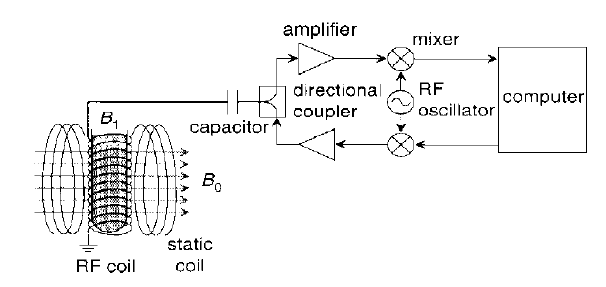
\includegraphics[scale=0.8]{gnc.png}
\caption{Our NMR Quantum Computer So Far}
\end{figure}
\end{center}

The basic process of creating an RF pulse is done by the RF coil, the pulsing action basically being an oscillating magnetic field(if you remember, $\mathbb{B}_1$) and a \textbf{solenoid} is used to create a static magnetic field, which is $\mathbb{B}_0$ in our case. The corresponding amplification circuit is used to make these resonance shifts "audible" enough for the quantum computer, along with another RF oscillator in parallel. Coming to our roadmap, they form a sort of a checklist, this procedure has been adapted from the paper~\cite{ethz}.
\clearpage
\subsection{DiVicenzo's Criteria}
So far, whatever implementation techniques we have seen, we can say that they are \textit{almost} always based on the conversions between the two Lie algebras discussed before. However, we cannot say that, this is the only mathematical correspondence that forms the basis for any quantum computer. For instance, Alexei Kitaev's ~\cite{kit}idea of using topological properties such as \textbf{braids etc,.} to create things such as \textbf{Topological quantum computers} is one such deviation from the common line of thought. To speak a bit more about them, topological quantum computers can be said to have very less \textbf{decoherence} when compared to other models, even the NMR computer. But, all of these models follow what is known as the \textit{DiVicenzo's Criteria} listed out by the pioneer David DiVicenzo in his seminal paper ~\cite{ddv1},
\begin{enumerate}
\item Every system that is supposed to be used as a quantum computer, must essentially have a \textbf{definite way of representing qubits}. In our case, it is obviously the spin of the nucleus that delimits this criterion.\\
\item Every system must have some sort of a mechanism to emulate the action that a quantum gate would do on paper. On paper, every gate is a unitary matrix. We must find\textbf{ a process which gives the same end result as that of operating this matrix on a state vector}. In our case, RF pulsing and \textit{defocusing} are the two techniques along with delayed signal pulses that help us achieve phase shifts etc. \\
\item Every system must be able to initialize in a state of uniform amplitudes for each qubit. There might be various initialization procedures for various algorithms itself, let alone computers. In the case of \textit{Grover's search algorithm}, we use the \textit{Walsh-Hadamard Gate} to initialize the n qubits into a state in which each one has the same amplitude. In our case, as we shall see, it is achieved automatically by the laws of statistical mechanics(remember Boltzmann distribution?~\cite{Feyn}), but we shall also see that, this causes an important issue with NMR quantum computers.\\
\item Every system must have access to the qubits for \textbf{measurement}, so that the final qubit states can be detected. Measurement plays a much more important role in quantum physics than in classical physics, which has been explained in section 2. In our case, this is done from the RF coil itself, by detecting the spin states. We shall describe the machinery in detail later on. 
\item Every system must be \textbf{fault-tolerant} to some extent. The main issue with quantum computers or for that matter, any quantum system is that slight noise from the environemnt might lead to what is known as \textbf{decoherence} which leads to the disturbance of the qubit and loss of information might take place. As explained before, Kitaev's model is fault tolerant to a large extent, whereas the NMR model faces an issue here. But this is not a very large issue as experimental coherence times have been measured upto the order of a few seconds~\cite{ethz} and this is not bad for a quantum state \textit{at room temperature}. 
\end{enumerate}
Let us tackle the issue of initialization in NMR computers first. We have already covered the part on implementing gates by RF pulses.
 
\bibliographystyle{plain}
\bibliography{nmrqc}
\end{document}